
\subsection{Flexible blokken}\label{felix}
Het is voor redacteuren mogelijk om blokken de plaatsen op pagina's. Hiermee krijgt de redacteur enige vrijheid over de indeling van de pagina. Hier zijn wel beperkingen van toepassing volgens het grafisch ontwerp.

Door met de muis over de grijze balk te gaan verschijnt er een tandwieltje, als je daarop klikt dan verschijnt er een optie \emph{Blok toevoegen}. Hier kan een keuze gemaakt worden om een enkel item weer te geven op de website, dit zijn \emph{Nodetypes}, of een aantal items, zoals bijvoorbeeld \emph{Het laatste nieuws}.

\begin{center}
	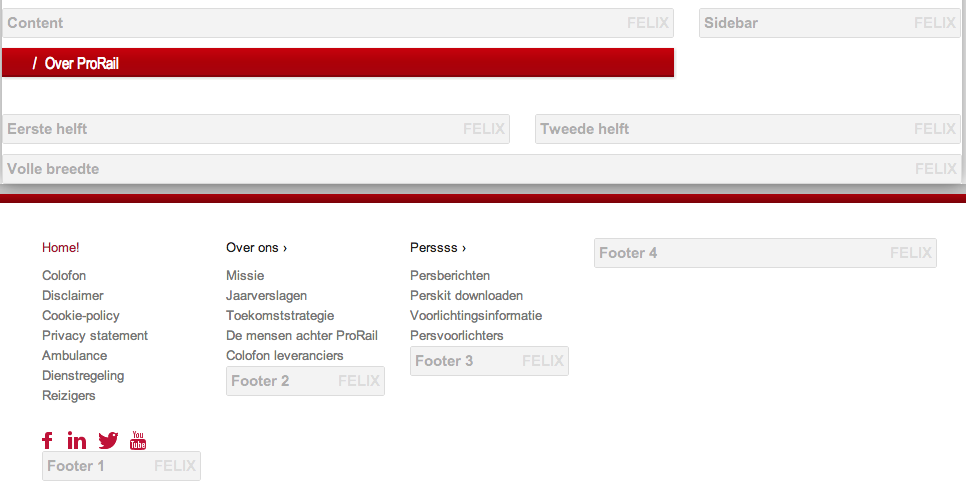
\includegraphics[width=\textwidth]{img/felix.png}
\end{center}